\section{Modelagem}\label{sec:modelagem}
\begin{frame}[allowframebreaks]{Modelagem}
	\begin{itemize}
		\setlength{\itemsep}{0.5em}
		\item<1-> Metodologia Kanban
		\item<1-> Personas
		\item<1-> Histórias de Usuário:
		\begin{itemize}
			\setlength{\itemsep}{0.5em}
			\item<1-> US01 -- Acessar o sistema
			\item<1-> US02 -- Buscar restaurante
			\item<1-> US03 -- Acessar cardápio
			\item<1-> US04 -- Filtrar cardápio
			\item<1-> US05 -- Favoritar restaurante
		\end{itemize}
	\end{itemize}
\end{frame}

\begin{frame}[allowframebreaks]{Banco de Dados}
	\centering
	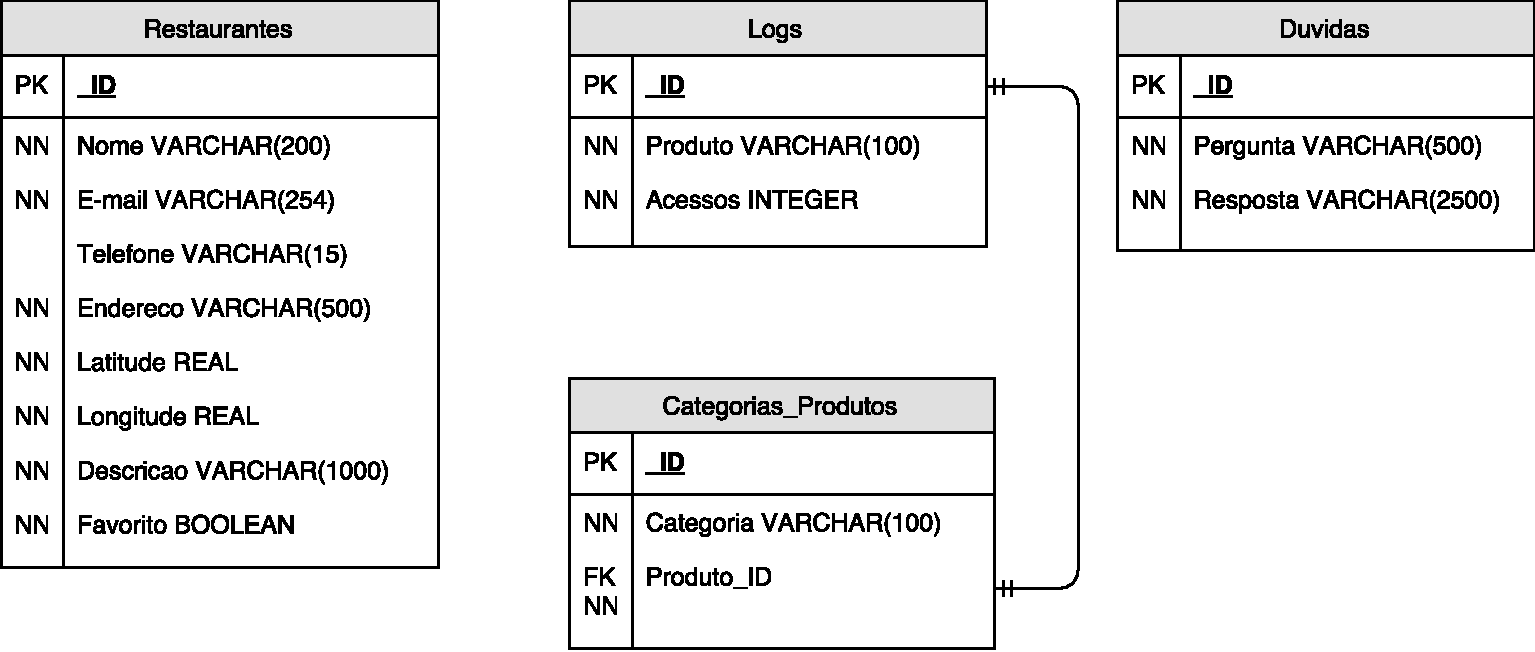
\includegraphics[width=1\linewidth]{../pdf/bd-slides.pdf}
\end{frame}

\begin{frame}{Fluxograma}
	\centering
	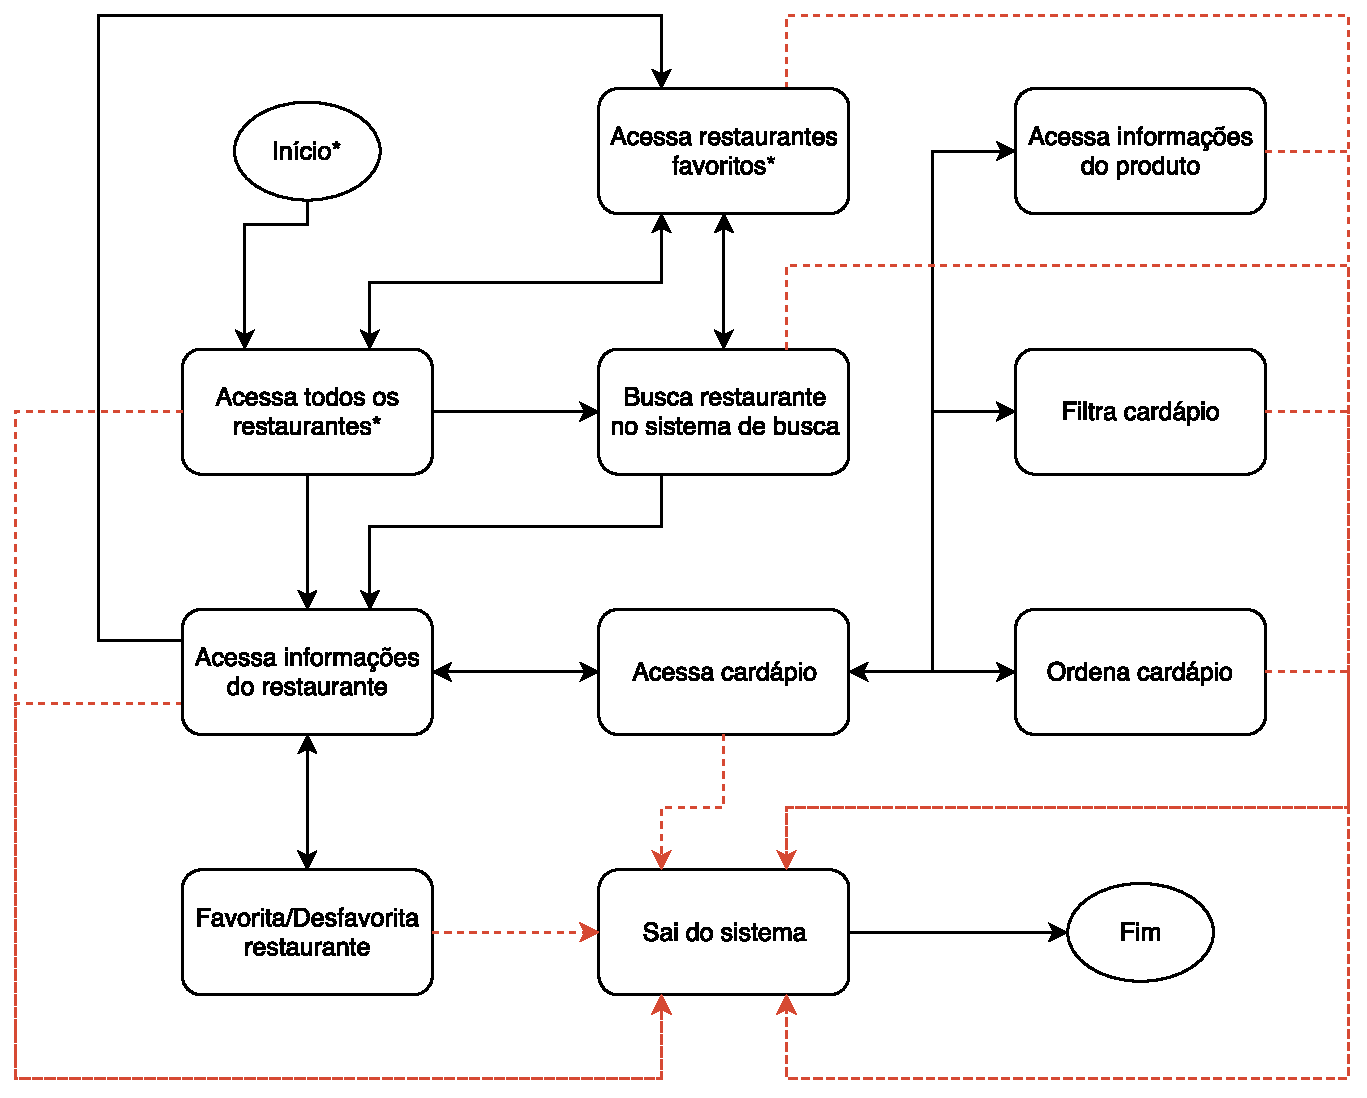
\includegraphics[width=0.8\linewidth]{../pdf/fluxograma-atual.pdf}
\end{frame}